%%%%%%%%%%%%%%%%%%%%%%%%%%%%% Define Article %%%%%%%%%%%%%%%%%%%%%%%%%%%%%%%%%%
\documentclass{article}
%%%%%%%%%%%%%%%%%%%%%%%%%%%%%%%%%%%%%%%%%%%%%%%%%%%%%%%%%%%%%%%%%%%%%%%%%%%%%%%

%%%%%%%%%%%%%%%%%%%%%%%%%%%%% Using Packages %%%%%%%%%%%%%%%%%%%%%%%%%%%%%%%%%%
\usepackage{geometry}
\usepackage{graphicx}
\usepackage{amssymb}
\usepackage{amsmath}
\usepackage{amsthm}
\usepackage{empheq}
\usepackage{mdframed}
\usepackage{booktabs}
\usepackage{lipsum}
\usepackage{graphicx}
\usepackage{color}
\usepackage{psfrag}
\usepackage{pgfplots}
\usepackage{bm}
\usepackage{float}
%%%%%%%%%%%%%%%%%%%%%%%%%%%%%%%%%%%%%%%%%%%%%%%%%%%%%%%%%%%%%%%%%%%%%%%%%%%%%%%

% Other Settings
% LTeX: language=es
\graphicspath{ {./resources/} }

%%%%%%%%%%%%%%%%%%%%%%%%%% Page Setting %%%%%%%%%%%%%%%%%%%%%%%%%%%%%%%%%%%%%%%
\geometry{a4paper}

%%%%%%%%%%%%%%%%%%%%%%%%%% Define some useful colors %%%%%%%%%%%%%%%%%%%%%%%%%%
\definecolor{ocre}{RGB}{243,102,25}
\definecolor{mygray}{RGB}{243,243,244}
\definecolor{deepGreen}{RGB}{26,111,0}
\definecolor{shallowGreen}{RGB}{235,255,255}
\definecolor{deepBlue}{RGB}{61,124,222}
\definecolor{shallowBlue}{RGB}{235,249,255}
%%%%%%%%%%%%%%%%%%%%%%%%%%%%%%%%%%%%%%%%%%%%%%%%%%%%%%%%%%%%%%%%%%%%%%%%%%%%%%%

%%%%%%%%%%%%%%%%%%%%%%%%%% Define an orangebox command %%%%%%%%%%%%%%%%%%%%%%%%
\newcommand\orangebox[1]{\fcolorbox{ocre}{mygray}{\hspace{1em}#1\hspace{1em}}}
%%%%%%%%%%%%%%%%%%%%%%%%%%%%%%%%%%%%%%%%%%%%%%%%%%%%%%%%%%%%%%%%%%%%%%%%%%%%%%%

%%%%%%%%%%%%%%%%%%%%%%%%%%%%%%% Plotting Settings %%%%%%%%%%%%%%%%%%%%%%%%%%%%%
\usepgfplotslibrary{colorbrewer}
\pgfplotsset{width=8cm,compat=1.9}
%%%%%%%%%%%%%%%%%%%%%%%%%%%%%%%%%%%%%%%%%%%%%%%%%%%%%%%%%%%%%%%%%%%%%%%%%%%%%%%

%%%%%%%%%%%%%%%%%%%%%%%%%%%%%%% Title & Author %%%%%%%%%%%%%%%%%%%%%%%%%%%%%%%%
\title{Proyecto Final de Informática}
\author{Integrantes}
%%%%%%%%%%%%%%%%%%%%%%%%%%%%%%%%%%%%%%%%%%%%%%%%%%%%%%%%%%%%%%%%%%%%%%%%%%%%%%%

\begin{document}
    \maketitle
    
\section{Programa de Inicio}

El programa de inicio utiliza un ciclo \emph{do} junto a una variable booleana \emph{run}, de esta manera se obtiene a un programa que continuara ejecutando a no ser que el valor de \emph{run} sea falso. 

\begin{figure}[h]
    \centering
        \centering
    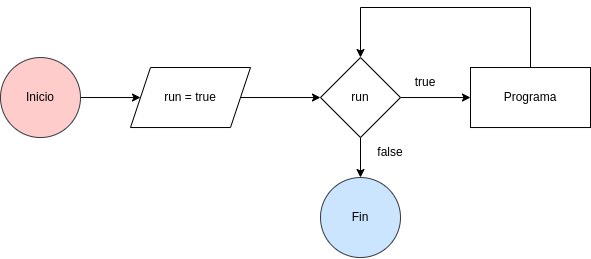
\includegraphics[width=8cm]{loop_inicio}
    \centering
        \centering
        \caption{Diagrama de Flujo del Ciclo Principal del Programa}
\end{figure}

Acá se le presenta al usuario una lista de programas disponibles y se captura la opción ingresada, este valor se evalúa con una estructura de control \emph{switch} para ejecutar cada ejercicio.

\begin{figure}[h]
    \centering
    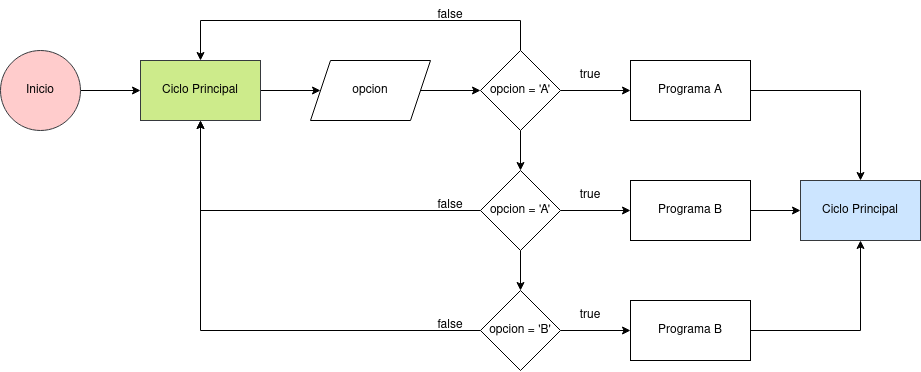
\includegraphics[width=8cm]{switch_programa}
    \caption{Diagrama de Flujo del Menú Principal}
\end{figure}

\section{Primer Programa}

El primer programa empieza capturando las 3 variables: \emph{a}, \emph{b} y \emph{c}, de tipo \emph{double} para no perder precisión al momento de calcular el área del triángulo. Estas variables son entonces evaluadas en un condicional para verificar si una de ellas es negativa o igual a 0, de ser verdad entonces se muestra el error ``¡Solo se aceptan valores positivos!'', de ser falso se continúa con otro condicional para evaluar si los valores ingresados crean un triángulo: \emph{(a + b) > c}, de ser falso se muestra el error: ``¡Los valores ingresados no crean un triángulo!''. Con estos valores ya evaluados se utiliza la \emph{fórmula de Herrón} para obtener el área del triángulo.

\begin{figure}[h]
    \centering
    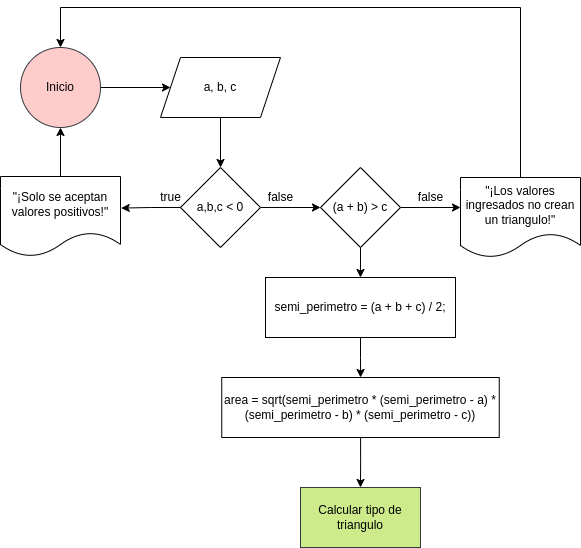
\includegraphics[width=8cm]{triangulo_area}
    \caption{Diagrama de Flujo del Calculador de Área de un Triángulo}
\end{figure}

Con el cálculo del área completo, se evalúa el tipo de triángulo con las medidas ingresadas.

\begin{figure}[h]
    \centering
    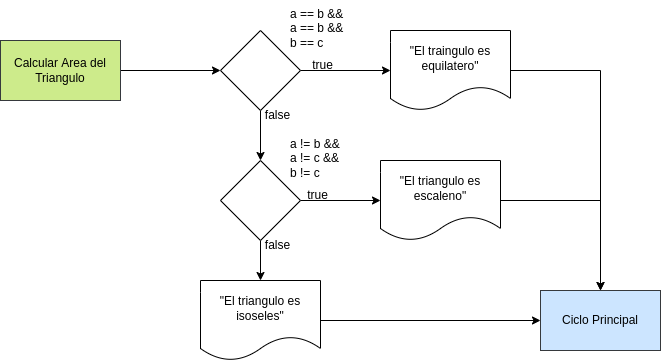
\includegraphics[width=8cm]{triangulo_tipo}
    \caption{Diagrama de Flujo del Calculador del Tipo de Triángulo}
\end{figure}

\section{Segundo Programa}

El calculador de promedio ponderado inicia solicitándole al usuario las 6 notas necesarias y su porcentaje sobre el promedio final de un estudiante.

\begin{figure}[H]
    \centering
    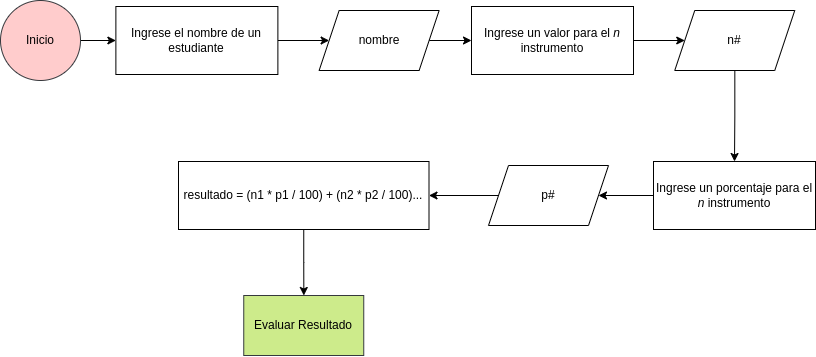
\includegraphics[width=8cm]{promedio_ponderado_calcular_resultado}
    \caption{Diagrama de Flujo del Cálculo del Promedio Ponderado}
\end{figure}

Con este resultado, se evalúa con un condicional si el estudiante ha pasado el curso con un promedio final mayor o igual a 70.

\begin{figure}[H]
    \centering
    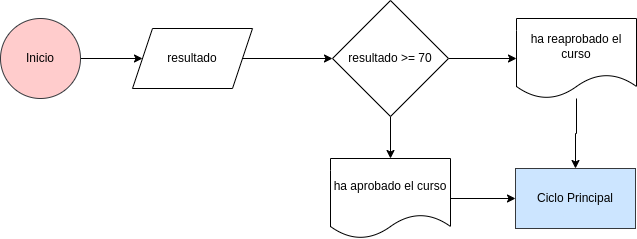
\includegraphics[width=8cm]{promedio_ponderado_salida}
    \caption{Diagrama de Flujo del Resultado Final del Promedio Ponderado}
\end{figure}

\section{Tercer Programa}

El contador de dígitos solícito el ingreso de un número, este número es enrealidad capturado en una variable de tipo \emph{String} para obtener su largo con la propiedad \emph{lenght}. Esta propiedad es usada para validar la cantidad de dígitos 

\begin{figure}[h]
    \centering
    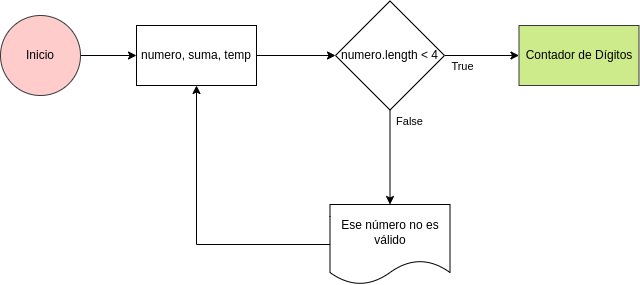
\includegraphics[width=8cm]{contador_digitos_validacion}
    \caption{Diagrama de la Validación del Programa Contador de Dígitos}
\end{figure}

Adicionalmente se usa esta propiedad para crear un ciclo \emph{for} con el cual se itera sobre cada carácter para poder sumarlo a una variable acumuladora llamada \emph{suma}, cabe a destacar el uso de la función \emph{stoi}, la cual permite convertir valores de tipo \emph{String} a valores de tipo numerales \emph{int} así como el uso de una variable ``temporal'' para guardar el valor actual del carácter por sumar.

\begin{figure}[H]
    \centering
    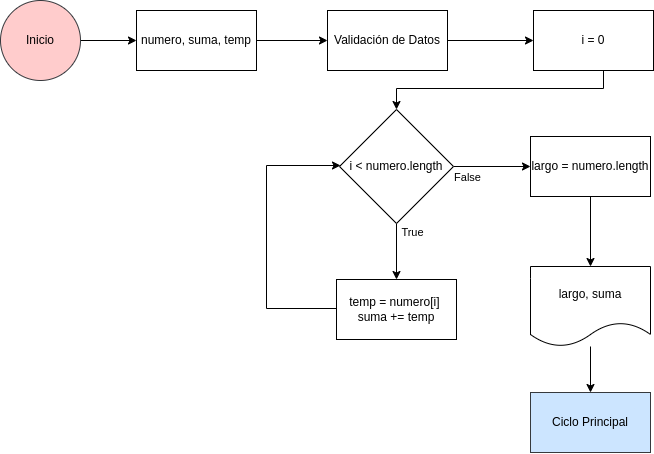
\includegraphics[width=8cm]{contador_digitos_ciclo}
    \caption{Diagrama de Flujo del Ciclo \emph{for} del Programa Contador de Dígitos}
\end{figure}

\section{Limitador de Intentos}

En el capítulo dedicado a cada programa se ha estado omitiendo el limitador de intentos máximos en caso de que el usuario ingrese una opción inválida al momento de seleccionar un programa por ejecutar, esto es logrado mediante una variable \emph{intentos}, la cual es reducida cada vez que el usuario ingresa un valor no esperado en el menú principal para que cuando este llegue a 3, se cierre el ciclo principal del programa poniendo el valor de la variable booleana \emph{run} en falso.

\begin{figure}[H]
    \centering
    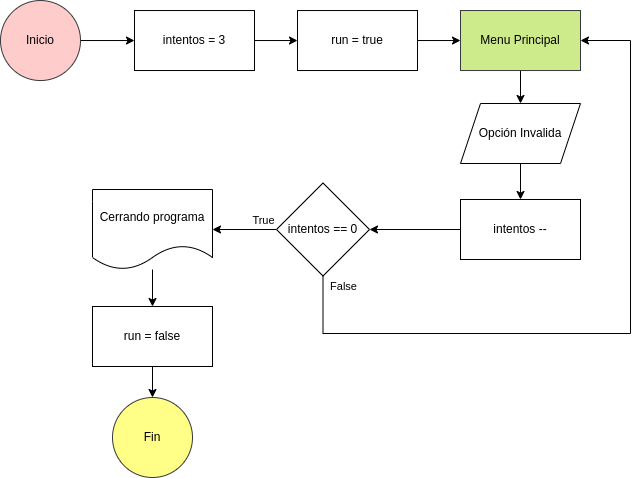
\includegraphics[width=8cm]{limitador_intentos_salida}
    \caption{Diagrama de Flujo del Programa de Salida}
\end{figure}

Cabe a destacar que este contador es restaurado cada vez que el usuario ingresa correctamente una opción presentada en el menú principal.

\begin{figure}[H]
    \centering
    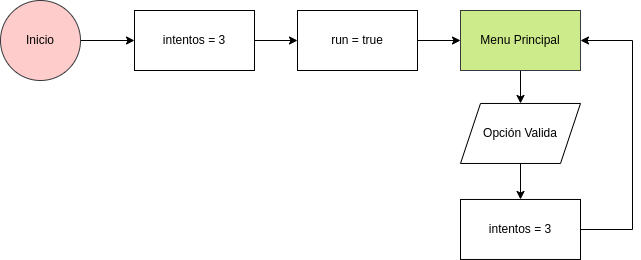
\includegraphics[width=8cm]{limitador_intentos_reinicio}
    \caption{Diagrama de Flujo del Limitador de Intentos}
\end{figure}

\section{Programa de Salida}

El programa de salida corresponde a un simple condicional que solicita confirmación del usuario para terminar la ejecución, si se confirma la salida del programa entonces se cambia el valor de la variable \emph{run} a falso y se cierra el ciclo principal del programa.

\begin{figure}[h]
    \centering
    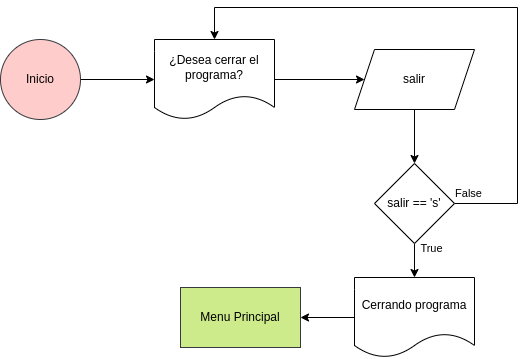
\includegraphics[width=8cm]{programa_salida}
    \caption{Diagrama de Flujo del Programa de Salida}
\end{figure}

\end{document}
